\documentclass[nobib]{tufte-handout}

\title{Föreläsning 11: Probabilistiska metoden $\cdot$ 1MA020}

\author[Vilhelm Agdur]{Vilhelm Agdur\thanks{\href{mailto:vilhelm.agdur@math.uu.se}{\nolinkurl{vilhelm.agdur@math.uu.se}}}}

%\date{20 februari 2023}


%\geometry{showframe} % display margins for debugging page layout

\usepackage{graphicx} % allow embedded images
  \setkeys{Gin}{width=\linewidth,totalheight=\textheight,keepaspectratio}
  \graphicspath{{graphics/}} % set of paths to search for images
\usepackage{amsmath}  % extended mathematics
\usepackage{booktabs} % book-quality tables
\usepackage{units}    % non-stacked fractions and better unit spacing
\usepackage{multicol} % multiple column layout facilities
\usepackage{lipsum}   % filler text
\usepackage{fancyvrb} % extended verbatim environments
  \fvset{fontsize=\normalsize}% default font size for fancy-verbatim environments

\usepackage{color,soul} % Highlights for text


\include{mathcommands.extratex}

\begin{document}

\definecolor{darkgreen}{rgb}{0.0627, 0.4588, 0.1451}

\maketitle% this prints the handout title, author, and date

\begin{abstract}
\noindent
I denna föreläsning ger vi fler tillämpningar av probabilistiska metoden på olika problem, praktiska och från andra delar av matematiken. Många men inte alla kommer handla om grafer.
\end{abstract}

\section{\texttt{min-bisection}-problemet}

Antag att vi har en grupp personer på en konferens, och vi vill dela upp dem i två lika stora grupper i olika rum. Vi vill att så många som möjligt som känner varandra skall få vara i samma rum -- ekvivalent vill vi alltså minimera mängden vänskapsband mellan rummen.\sidenote[][]{
  Ett annat sätt att motivera det här problemet är att vi har en graf som är för stor för att lagra i minnet på en enda dator, så vi vill använda två datorer och låta var och en av dem lagra hälften. Så länge vad vi vill räkna ut bara handlar om noder på en av de två datorerna kan vi räkna lokalt -- men om vi vill räkna ut något som involverar kanter mellan de två maskinerna måste de kommunicera med varandra, vilket är långsamt.
  
  För att kunna göra snabba beräkningar vill vi alltså hitta ett sätt att dela upp vår graf så att det inte går så många kanter mellan de två delarna. Det här är ett problem som behöver lösas i praktiken, även om man ofta då har fler än två datorer och behöver hitta en minimal $k$-partition av grafen istället.}

\begin{definition}
  Givet en graf $G = (V, E)$ på $2n$ noder är \texttt{min-bisection} problemet att hitta en minimal bisektion av $G$, alltså att hitta en delmängd $A \in \binom{V}{n}$ som minimerar antalet kanter mellan $A$ och $A^c$. Formellt skriver vi
  $$\min_{A \in \binom{V}{n}} \abs{E(A, A^c)}$$
  där $E(A, A^c)$ alltså är mängden av kanter mellan $A$ och dess komplement $A^c$.
\end{definition}

Hur väl kan vi lösa det här problemet? Ibland är det väldigt svårt -- om vi har fyra personer där alla känner alla, alltså grafen är den fullständiga grafen $K_4$, kommer vi alltid att ha $4$ av $6$ kanter mellan de två delarna.

\begin{figure}
  \centering
  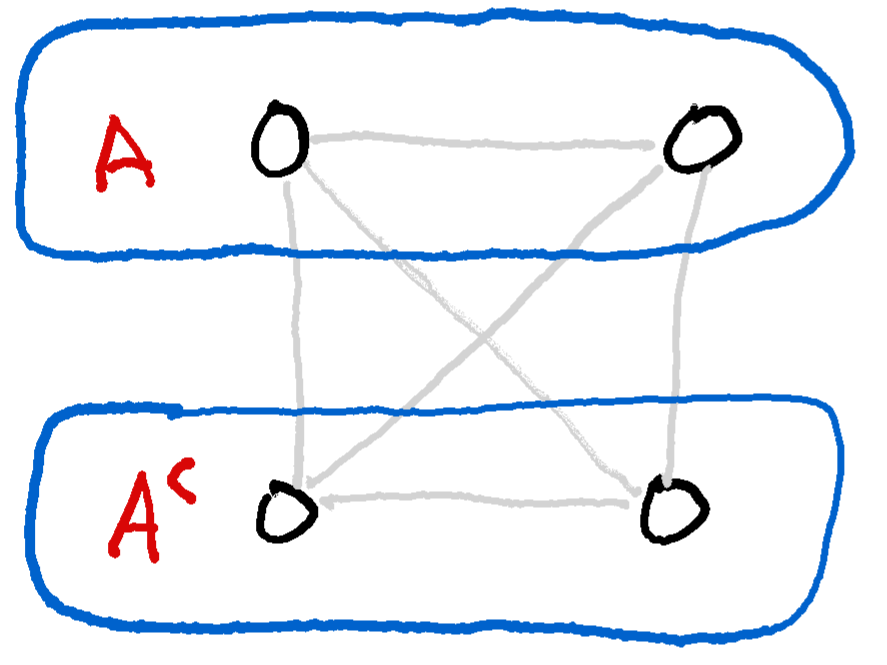
\includegraphics[width=0.5\textwidth]{graphics/K4_min_bisection.png}
  \caption{$K_4$ uppdelad i en bisektion. På grund av symmetrin i grafen är detta så klart enda sättet att dela upp den.}
\end{figure}

Det visar sig att nyckelegenskapen för att kunna göra det här väl är att grafen inte får ha för många kanter relativt antalet noder -- vilket väl inte är allt för överraskande, om man tänker efter.

För att kunna ge en precis variant av det påståendet behöver vi en definition och en sats från grafteorin. Vi utelämnar beviset för satsen, eftersom det inte använder någon sannolikhetsteori.

\begin{definition}
  En Hamiltoncykel i en graf är en cykel som innehåller alla noder exakt en gång. Givet $G = ([n],E)$ kan vi alltså se det som en permutation $\sigma \in S_n$ sådan att $\{\sigma(i),\sigma(i+1)\}$ är en kant för alla $i$, och $\{\sigma(1), \sigma(n)\} \in E$.
\end{definition}

\begin{theorem}[Diracs sats]\sidenote[][]{Inte fysikern, en annan Dirac.}
  Om varje nod i $G = ([n], E)$ har grad\sidenote[][]{Antal grannar.} minst $\frac{n}{2}$ så finns det en Hamiltoncykel i $G$.
\end{theorem}

Vi kan använda denna sats för att bevisa följande resultat:

\begin{proposition}
  Låt $G = ([n], E)$ vara en graf på ett jämnt antal noder, och antag att varje nod har grad högst $\frac{n}{2}$. Då existerar det en delmängd $A \in \binom{[n]}{n/2}$ sådan att
  $$\abs{E(A, A^c)} \leq \frac{\abs{E}}{2}.$$ 

  \begin{proof}
    Låt $G'$ vara komplementgrafen till $G$ -- alltså grafen där det finns en kant mellan varje par av noder som \emph{inte} har en kant mellan sig i $G$, och som inte har en kant mellan par av noder som har en kant i $G$.

    Vi ser enkelt att graden av $i$ i $G'$ är precis $n$ minus graden av $i$ i $G$, så eftersom $d_i \leq n/2$ i $G$ måste $d_i' \geq n/2$ i $G'$. Alltså kan vi tillämpa Diracs sats och hitta en Hamiltoncykel $\sigma$ i komplementgrafen $G'$.

    Vi kan nu använda denna Hamiltoncykel för att para ihop noder i $G$ -- vi matchar $\sigma(1)$ med $\sigma(2)$, $\sigma(3)$ med $\sigma(4)$, och så vidare. Eftersom detta var en Hamiltoncykel i komplementgrafen är vi alltså garanterade att vi aldrig parar ihop två noder som har en kant mellan sig.

    Vi kan nu skapa oss en slumpmässig delmängd $A \in \binom{[n]}{n/2}$ genom att, för varje par, slumpmässigt välja en av de två noderna att ha med i $A$, och låta den andra vara utanför $A$. Denna delmängd kommer ha rätt storlek eftersom vi väljer en nod ur varje par, så vi måste få precis hälften av noderna.

    Låt oss nu räkna ut väntevärdet av $E(A, A^c)$. Vi får att
    \begin{align*}
      \E{E(A, A^c)} &= \E{\sum_{e \in E} \ind{e \in E(A, A^c)}}\\
      &= \sum_{e \in E} \E{\ind{e \in E(A, A^c)}}\\
      &= \sum_{e \in E} \Prob{e \in E(A, A^c)}.
    \end{align*}

    Vad är sannolikheten att en viss fix kant $e = \{u, v\}$ går mellan $A$ och $A^c$? Jo, det händer precis när vi valt att $u \in A$ och $v \in A^c$, eller vice versa. Så vi kan räkna att\sidenote[][]{Vi utnyttjar att de är disjunkta händelser för att gå från $\Prob{(u \in A, v \in A^c) \cup (u \in A^c, v \in A)}$ till summan av de två sannolikheterna.}
    $$\Prob{\{u,v\} \in E(A, A^c)} = \Prob{u \in A, v \in A^c} + \Prob{u \in A^c, v \in A}.$$
    
    Nyckeln nu, och anledningen att vi krånglade med Hamiltoncykeln och matchningen, är att händelserna $u\in A$ och $v\in A^c$ måste vara oberoende. Om $u$ är i $A$ eller inte beror på en myntsingling vi gjorde för $u$ och noden den parades ihop med -- så om vi kallar dess partner för $w$ så är $u \in A$ och $w \in A$ inte oberoende, men för alla $v \neq w$ är $u \in A$ oberoende från $v \in A$.

    Så hur vet vi att vårt par $u, v$ i vår räkning inte råkar ha parats ihop, så att händelserna att de ligger i $A$ inte är oberoende? Jo, vi vet ju att det går en kant mellan $u$ och $v$ -- det är därför vi är intresserade av dem -- men det går ingen kant mellan något par av noder vi parat ihop.

    Alltså kan vi fortsätta vår räkning och få
    \begin{align*}
      \Prob{\{u,v\} \in E(A, A^c)} &= \Prob{u \in A, v \in A^c} + \Prob{u \in A^c, v \in A}\\
      &= \Prob{u \in A}\Prob{v \in A^c} + \Prob{u \in A^c}\Prob{v \in A}\\
      &= \frac{1}{2}\cdot\frac{1}{2} + \frac{1}{2}\cdot\frac{1}{2} = \frac{1}{2}
    \end{align*}
    och alltså har vi att
    \begin{align*}
      \E{E(A,A^c)} &= \sum_{e \in E} \Prob{e \in E(A, A^c)}\\
      &= \sum_{e \in E} \frac{1}{2} = \frac{\abs{E}}{2}.
    \end{align*}

    Enligt vårt sedvanliga argument att väntevärdet omöjligen kan vara mindre än varje specifikt värde måste det alltså finnas ett specifikt $A$ sådant att $E(A, A^c) \leq \E{E(A,A^c)} = \frac{\abs{E}}{2}$ och vi har bevisat satsen.
  \end{proof}
\end{proposition}

\section{ACNSL-olikheten och VLSI}

I nästan varje sak vi gjort som involverat grafer så har vi ritat bilder av grafen på tavlan, och försökt göra dessa bilder så tydliga som möjligt. Vi väljer att rita dem så att kanterna inte korsar varandra om de inte absolut måste.

Detta leder oss till en faktisk matematisk fråga: Givet en graf $G$, hur få korsningar mellan kanter kan vi rita den med?

\begin{definition}
  En graf $G$ som vi kan rita helt utan att några kanter korsar varandra kallas för \emph{planär}. I allmänhet betecknar vi det minimala antalet korsningar av kanter i en ritning av $G$ med $cr(G)$.\sidenote[][]{Från engelskans \emph{crossing number}.}
\end{definition}

Låt oss återigen ge ett lemma som vi inte bevisar.

\begin{lemma}\label{newtons_formula_lemma}
  Det gäller för alla grafer $G = (V, E)$ att
  $$cr(G) \geq \abs{E} - 3\abs{V} + 6.$$

  \begin{proof}
    Utelämnas.\sidenote[][]{Idén i beviset är att använda Eulers formel och sedan resonera om att ta bort kanter som korsar andra kanter:
    \begin{lemma}[Eulers formel]
      Om $G = (V, E)$ är planär är
      $$3\abs{V} - 6 \geq \abs{E}.$$
    \end{lemma}
    
    Hur bevisar man Eulers formel? Den är ett specialfall av Eulerkarakteristiken av en polyeder. För en väldigt lång och intressant diskussion av just hur man bevisar detta, och primärt vad det faktiskt innebär att bevisa något, se Imre Lakatos bok \emph{Proofs and Refutations}, som handlar enbart om just det.
    
    Vill man ha en kortare diskussion av detta kan man se till exempel föreläsningsanteckningarna för kursen i grafteori vid detta universitet -- just ämnet med planära grafer är en av de vackrare delarna av den kursen.}
  \end{proof}
\end{lemma}

Anledningen att vi ger den här olikheten är att vi faktiskt kan enkelt härleda en starkare version av samma olikhet med ett probabilistiskt trick. Såsom mycket annan modern matematik är listan av upptäckare lång -- till skillnad från förr i tiden görs merparten av all matematik i samarbeten numera.

\begin{theorem}[Ajtai-Chvatal-Newborn-Szemerédi-Leighton (ACNSL)]
  För varje graf $G = (V,E)$ gäller det att, om $\abs{E} \geq 4\abs{V}$ så är
  $$cr(G) \geq \frac{\abs{E}^3}{64\abs{V}^2}.$$

  \begin{proof}
    För att förenkla vår notation, låt $n = \abs{V}$ och $e = \abs{E}$. Tag ett godtyckligt $p \in (0,1)$.

    Vad vi vill göra är att studera en slumpmässig delgraf $H$ till $G$, som ges av att varje nod i $G$ är med i $H$ med sannolikhet $p$, och varje kant är med om bägge dess ändpunkter är med i $H$.\sidenote[][]{Detta kallas i allmänhet \emph{nodperkolation} på $G$. Perkolationsteori är ett stort ämne i sannolikhetsteorin, med kopplingar till fysiken -- man brukar tänka sig det som en modell för hur vatten sipprar genom sten. Således namnlikheten till perkolatorkaffe.}

    Vi får av Lemma \ref{newtons_formula_lemma} att
    $$cr(H) \geq \abs{E(H)} - 3\abs{V(H)} + 6.$$
    Eftersom denna likhet gäller för \emph{alla} utfall måste den också gälla om vi tar väntevärdet på bägge sidorna,\sidenote[][]{
      Vi kan formulera detta som ett lemma:
      \begin{lemma}
        Om $X(\omega) \geq Y(\omega)$ för varje $\omega \in \Omega$ så är $\E{X} \geq \E{Y}$.

        \begin{proof}
          Vi räknar att
          \begin{align*}
            \E{X} &= \sum_{\omega \in \Omega} X(\omega)\mu(\omega)\\
            &\geq \sum_{\omega \in \Omega} Y(\omega)\mu(\omega) = \E{Y}.
          \end{align*}
        \end{proof}
      \end{lemma}
    } så från väntevärdets linjäritet får vi alltså att
    \begin{equation}\label{eq:H_expectations_ineq}
      \E{cr(H)} \geq \E{\abs{E(H)}} - 3\E{\abs{V(H)}} + 6.
    \end{equation}

    Så låt oss studera vardera av dessa väntevärden. Så vi räknar att
    \begin{align*}
      \E{\abs{V(H)}} &= \E{\sum_{v \in V(G)} \ind{v \in V(H)}}\\
      &= \sum_{v \in V(G)} \Prob{v \in V(H)} = \abs{V(G)}p = np,
    \end{align*}
    och
    \begin{align*}
      \E{\abs{E(H)}} &= \E{\sum_{\{u,v\} \in E(G)} \ind{\{u,v\} \in E(H)}}\\
      &= \sum_{\{u,v\}\in E(G)} \Prob{\{u,v\} \in E(H)}\\
      &= \sum_{\{u,v\}\in E(G)} \Prob{u \in V(H), v \in V(H)}\\
      &= \sum_{\{u,v\}\in E(G)} \Prob{u \in V(H)}\Prob{v \in V(H)} = \abs{E(G)}p^2 = ep^2.
    \end{align*}

    Hur hanterar vi $\E{cr(H)}$? Jo, vi tar en ritning av $G$ som har precis $cr(G)$ korsningar, och räknar hur många av de korsningarna som är kvar när vi suddat ut alla noder och kanter utanför $H$. Det här ger oss en övre begränsning på $cr(H)$ -- det är ju tänkbart att det finns en bättre ritning av $H$ än att bara rita varje nod och kant på samma sätt som de var ritade i $G$.

    För att korsningen skall vara kvar krävs det så klart att bägge kanterna i korsningen är kvar -- och vi har sett att sannolikheten att en enda kant är kvar är $p^2$, så eftersom kanter är kvar oberoende av varandra\sidenote[][]{Förutom om de utgår från samma nod -- men vi kan aldrig tvingas att rita två kanter som utgår från samma nod så att de korsas. (Detta är ganska uppenbart men inte helt trivialt -- fundera ett ögonblick på varför det är sant.)} är sannolikheten att en korsning blir kvar $p^4$.

    Så enligt samma logik som i de andra fallen får vi att $\E{cr(H)} \leq cr(G)p^4$, så om vi sätter in resultatet av våra räkningar i \eqref{eq:H_expectations_ineq} så får vi att
    $$p^4cr(G) \geq p^2e - 3pn + 6$$
    så om vi nu väljer $p = \frac{4n}{e}$ så får vi alltså
    $$\left(\frac{4n}{e}\right)^4 cr(G) \geq \frac{(4n)^2}{e} - 3\frac{4n^2}{e} + 6 > \frac{(4n)^2}{e} - 3\frac{4n^2}{e}$$
    vilket förenklar till påståendet vi sade vi skulle bevisa.
  \end{proof}
\end{theorem}

Varför är det här ett intressant problem? Att rita grafer med så få korsningar som möjligt är inte bara ett estetiskt problem när man ritar saker på en blackboard, utan också ett praktiskt problem när man skall designa kretskort.

Kretskorten har nämligen många olika komponenter, som vi kan tänka oss som noder, som skall kopplas ihop med varandra. Så länge inte kopplingarna korsar varandra kan man helt enkelt måla dit dem, men om de skall korsa behöver man göra något mer komplicerat. Alltså är det av praktiskt intresse att hitta sätt att rita grafer som minimerar antalet korsningar -- problemet i allmänhet med kretskortsdesign kallas för VLSI (Very Large Scale Integration).

\section{Oberoende mängder i triangelfria grafer}

Vi har redan innan visat resultat om antalet oberoende mängder i en graf -- förra föreläsningen visade vi Caro-Weis sats, och i en övning ger vi ett annat resultat om oberoende mängder med ett annat bevis.

Låt oss nu ge ytterligare ett resultat om oberoende mängder, denna gång under antagandet att grafen inte har några trianglar. Att detta borde hjälpa oss att hitta större oberoende mängder är någorlunda intuitivt -- i en triangel kan vi ju bara ha med högst ett av de tre hörnen i vår oberoende mängd. Att inte innehålla någon triangel är dessutom en begränsning på antalet kanter grafen kan innehålla 
\sidenote[][]{Detta är Turáns sats -- en graf på $n$ noder som inte innehåller några trianglar kan inte ha mer än $\frac{n^2}{4}$ kanter. 

Detta maximala antal kanter uppnås för övrigt av att ta en graf som har två grupper $A$ och $B$ av $n/2$ noder var, och rita varje kant $\{a,b\}$ mellan $A$ och $B$ och inga kanter inuti varken $A$ eller $B$.

En sådan graf kallas för \emph{bipartit}, och en sådan har en väldigt stor oberoende mängd -- både $A$ och $B$ blir ju oberoende i denna graf.}
-- och desto färre kanter desto enklare blir det ju att hitta en oberoende mängd, eftersom varje kant säger att ``du får bara ta en av dessa två noder till din oberoende mängd''.

Så resultatet vi ger säger oss något om hur stor oberoende mängd vi kan få om vi inte innehåller en triangel, och dessutom vet att varje nod har låg grad.

\begin{theorem}[Ursprungligen av Ajtai-Komlós-Szemerédi, bevis av Shearer]\label{thm:shearer_triangle_free_indep_set}
  Låt $G = (V, E)$ vara en triangelfri graf på $n$ noder, och skriv $\Delta = \max_{v \in V} d_v$ för den maximala graden av en nod i $G$. Då finns det en oberoende mängd $S \subseteq V$ sådan att
  $$\abs{S} \geq n\frac{\log_2(\Delta)}{8\Delta}.$$
\end{theorem}

Låt oss bryta ut den centrala idén i beviset av det här i ett lemma, bevisa det, och sedan använda lemmat för att bevisa satsen. I beviset kommer vi välja en slumpmässig oberoende mängd\sidenote[][]{Vi väljer alltså varje oberoende mängd med samma sannolikhet -- för det mesta brukar vi ju välja våra slumpvariabler som likformigt fördelade på en mängd vi förstår oss på väl, men det är så klart tillåtet att göra på detta viset också.} $S$, och sedan visa en nedre begränsning av $\E{\abs{S}}$. Som vanligt vill vi studera vårt problem ``lokalt'', runt en enda nod -- så frågan vi vill ställa oss är: Om vi vet hur $S$ ser ut överallt utom i $v$ och dess grannar, vad kan vi säga om sannolikheten att $v \in S$? Och hur många av $v$s grannar ligger i genomsnitt i $S$?

Det visar sig att vi kan svara på dessa frågor, och ge exakta uttryck, men det kräver en del notation för att kunna göra det -- formuleringen av lemmat blir nästan lika lång som beviset.

\begin{lemma}
  Låt $G = (V, E)$ vara en triangelfri graf på $n$ noder, och låt $S$ vara en likformigt slumpmässig oberoende mängd i $G$.

  Låt oss, för varje nod $v \in V$, skriva 
  $$H_v = G \setminus (v \cup N(v))$$
  så att $H_v$ alltså är hela $G$ förutom just $v$ och dess grannar.
  
  Vi skriver $N_v(S)$ för mängden av grannar till en nod i $S \cap H_v$,\sidenote[][-1.5cm]{Alltså mängden noder vi inte kan lägga till till $S \cap H_v$ utan att den slutar vara en oberoende mängd.} alltså
  $$N_v(S) = \bigcup_{v \in S \cap H_v} N(v)$$
  och vi låter $P_v = N(v) \setminus N_v(S)$ -- så att $P_v$ är mängden av grannar till $v$ som hade kunnat läggas till till $S$.

  Då gäller det för varje $v$ att
  \sidenote[][-2.5cm]{Den uppmärksamma läsaren bör vara skeptisk mot vad vi just skrivit här, både i vänster och höger led.
  
  I vänster led skrev vi en betingad sannolikhet där vi betingade på en \emph{slumpvariabel}, men vi har ju definierat betingade sannolikheter som att vi betingar på \emph{händelser}.
  
  I höger led påstår vi sedan att denna betingade sannolikhet blir lika med ett uttryck som inte är ett tal utan en \emph{slumpvariabel} -- $S$ är ju slumpmässig, så varje uttryck som innehåller $S$ kommer ju också vara slumpmässigt tills vi skriver ett $\Prob{\,}$ eller $\E{\,}$ för att omvandla det till ett tal.
  
  Det finns definitioner som gör det här helt väldefinierat, men vi kan nöja oss med att betrakta detta som en läsligare notation för påståendet att, för varje oberoende mängd $W\subseteq H_v$, så är
  $$\Prob{v \in S \given S \cap H_v = W} = \left(2^{\abs{P_v}} + 1\right)^{-1}.$$
  
  I detta påstående, när vi valt ett $W$, blir ju $S \cap H_v = W$ en händelse, och höger led blir bara ett tal eftersom $W$ är en fix mängd. Så detta är väldefinierat enligt våra definitioner.}
  $$\Prob{v \in S \given S \cap H_v} = \frac{1}{2^{\abs{P_v}} + 1}.$$
  och
  $$\E{\abs{N_v \cap S} \given S\cap H_v} = \frac{\abs{P_v}}{2 + 2^{1-\abs{P_v}}}.$$

  \begin{proof}
    Det är mycket notation i formuleringen av detta lemma, men beviset är faktiskt rätt så enkelt, i alla fall när man har rätt bild i huvudet av vad som pågår -- att studera Figur \ref{fig:triangle_free_graph} först för att förstå notationen innan man ger sig in i beviset är nog klokt.

    \begin{figure}
      \centering
      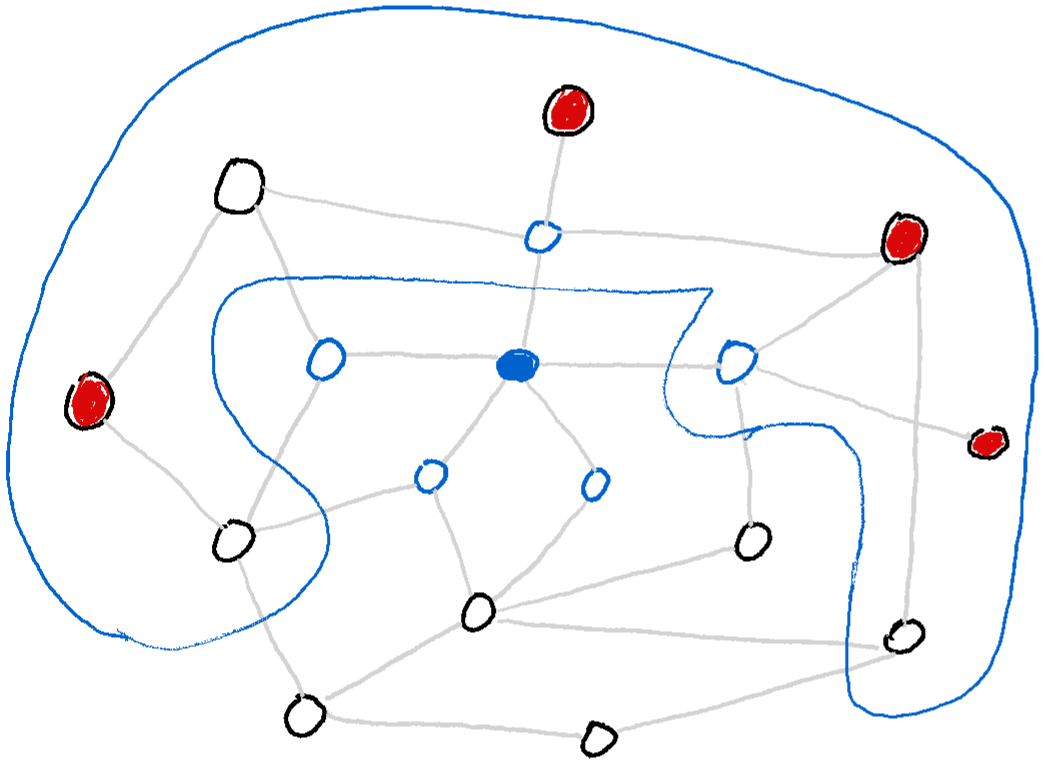
\includegraphics[width=0.9\textwidth]{graphics/independent_sets_in_triangle_free_graphs.png}
      \caption{En triangelfri graf, med noden $v$ ifylld blå, noderna i $N(v)$ ihåligt blå, noder i $H_v$ svarta, noder i $S \cap H_v$ ifyllda i rött, och mängden $N_v(S)$ inringad med en blå cirkel.}
      \label{fig:triangle_free_graph}
    \end{figure}

    Vad vi behöver svara på är följande fråga: Givet att vi vet vilka noder i $H_v$ som är med i $S$, hur många olika sätt kan vi utvidga $S$ till hela $G$, alltså inklusive $v \cup N(v)$, och hur många av dessa sätt har $v \in S$?

    Den senare delen av frågan är enkel att besvara -- så snart vi lagt in $v$ i $S$ så får så klart inga av dess grannar vara med i $S$, så det finns exakt ett sätt att utvidga $S$ från $H_v$ till hela $G$ sådant att $v \in S$.

    Hur många sätt finns det att utvidga $S$ om vi säger att $v \not\in S$? Jo, för varje granne till $v$ ligger den antingen i $N_v(S)$, och får inte läggas till, eller så ligger grannen i $N_v(S)^c$ och vi får lov att lägga till den. 
    
    Eftersom grafen inte innehåller några trianglar finns det inga kanter mellan något par av noder i $N(v)$ -- alltså kan våra val av noder ur $N(v) \cap N_v(S)^c$ att lägga till till $S$ inte blockera varandra, så varje delmängd till $N(v) \cap N_v(S)^c$ är ett giltigt val.

    Alltså finns det $2^{\abs{N(v) \cap N_v(S)^c}}$ sätt att utvidga $S$ till hela $G$ sådana att $v \not \in S$.

    Eftersom $S$ var likformigt fördelad på mängden av oberoende mängder måste varje av dessa alternativ vara lika sannolikt, och alltså är sannolikheten att vi väljer det enda alternativet där $v \in S$ precis
    $$\frac{1}{2^{\abs{N(v) \cap N_v(S)^c}} + 1}$$
    såsom vi önskade bevisa.

    För att räkna ut väntevärdet av antalet noder i $N(v)$ som ligger i $S$ kan vi räkna likadant. Först noterar vi att $N(v) \cap S = P_v \cap S$ -- en nod som inte ligger i $P_v$ har redan en granne i $S$, så den kan omöjligen hamna i $S$.
    
    Vi har sett att det finns totalt $2^{\abs{P_v}} + 1$ möjliga värden för $P_v \cap S$, och alla är lika sannolika, så
    \begin{align*}
      \E{\abs{N(v) \cap S} \given S \cap H_v} &= \E{\abs{P_v \cap S} \given S \cap H_v}\\
      &= 0\cdot \Prob{v \in S \given S \cap H_v}\\
      &\qquad + \sum_{Q \subseteq P_v} \abs{Q}\Prob{P_v \cap S = Q \given S \cap H_v}\\
      &= \sum_{i=0}^{\abs{P_v}} \sum_{\substack{Q \subseteq P_v\\\abs{Q} = i}} \frac{i}{2^{\abs{P_v}} + 1}\\
      &= \frac{1}{2^{\abs{P_v}} + 1}\sum_{i=0}^{\abs{P_v}} i\binom{\abs{P_v}}{i}\\
      &= \frac{\abs{P_v}\,\, 2^{\abs{P_v} - 1}}{2^{\abs{P_v}} + 1} = \frac{\abs{P_v}}{2^{1-\abs{P_v}} + 2}
    \end{align*}
    vilket är precis vad vi ville bevisa.\sidenote[][]{För att ta oss från näst sista raden till sista raden använde vi oss av likheten
    $$\sum_{k=0}^{n} k\binom{n}{k} = n 2^{n-1}.$$
    
    Att bevisa denna likhet med ett kombinatoriskt bevis är en av våra extraövningar.}
  \end{proof}
\end{lemma}

Med detta resultat i handen kan vi nu ge vårt bevis för Teorem \ref{thm:shearer_triangle_free_indep_set}.

\begin{proof}[Bevis av Teorem \ref{thm:shearer_triangle_free_indep_set}]
  Om $\Delta < 16$ följer resultatet av Caro-Weis sats, så vi antar att $\Delta \geq 16$. Låt $S$ vara en likformigt slumpmässig oberoende mängd i $G$.

  Vi definierar, för varje $v \in V$, en slumpvariabel $X_v$ som
  $$X_v = \Delta\ind{v \in S} + \abs{N(v) \cap S}.$$

  Låt oss nu studera väntevärdet av summan av dessa $X_v$. Vi ser att det är sant, för alla utfall, att
  \begin{align*}
    \sum_{v \in V} X_v &= \sum_{v \in V} \Delta\ind{v \in S} + \abs{N(v) \cap S}\\
    &= \Delta\abs{S} + \sum_{v \in V} \abs{N(v) \cap S}\\
    &= \Delta\abs{S} + \sum_{w \in S} \abs{N(w)}.
  \end{align*}

  Vad hände i det sista steget? Jo, vi observerar att de två summorna bara är olika sätt att räkna samma sak -- antalet kanter mellan en nod i $S$ och en utanför $S$. I den första summan summerar vi över alla noder, och räknar antalet kanter från den noden till en nod i $S$, och i den andra summan summerar vi över alla noder i $S$ och räknar antalet kanter från den till någonting utanför $S$.

  Vi vet också att alla noder har grad högst $\Delta$, så att $\abs{N(w)} \leq \Delta$ för alla $w$. Alltså måste vi ha från vår räkning att
  $$\sum_{v \in V} X_v = \Delta\abs{S} + \sum_{w \in S} \abs{N(w)} \leq \Delta\abs{S} + \sum_{w \in S} \Delta = 2\Delta\abs{S}.$$

  Så om vi kan hitta en nedre begränsing på $\sum_{v\in V} X_v$ kommer vi alltså att ha en nedre begränsning på $\abs{S}$, vilket ju är vad vi är ute efter.

  Så låt oss studera $\E{X_v}$. Vi kan använda vårt lemma och lagen om total sannolikhet 
  \sidenote[][]{Här ser vi en av de stora anledningarna till att använda våra betingningar på slumpvariabler istället för på händelser. Hade vi betingat på händelsen att $S \cap H_v = W$ för olika $W$ hade vi behövt skriva
  \begin{align*}
    \E{X_v} = \sum_{\substack{W\\\text{ober. mgd. i } H_v}} \substack{\E{X_v \given S \cap H_v = W}\cdot\\\qquad\cdot\Prob{S \cap H_v = W}},
  \end{align*}
  vilket ju är ett uttryck så stort att vi knappt kan formatera det i marginalen!
  
  Med vårt alternativa skrivsätt kan vi formulera lagen om total sannolikhet som att den säger att
  $$\E{A} = \E{\E{A \given B}}$$
  för varje par av slumpvariabler $A$ och $B$ -- en mycket renare formulering, som ger kortare formler.}
  för att få ut att
  \begin{align*}
    \E{X_v} &= \E{\E{X_v \given S \cap H_v}}\\
    &= \E{\E{\Delta\ind{v \in S} + \abs{N_v \cap S} \given S \cap H_v}}\\
    &= \E{\Delta\Prob{v \in S \given S \cap H_v} + \frac{\abs{P_v}}{2^{1-\abs{P_v}} + 2}}\\
    &= \E{\frac{\Delta}{2^{\abs{P_v}} + 1} + \frac{\abs{P_v}}{2^{1-\abs{P_v}} + 2}}
  \end{align*}

  Vad vi vill göra nu är att bevisa att uttrycket inuti väntevärdet är större än $\frac{1}{4}\log_2(\Delta)$ för \emph{alla} utfall. Antag alltså för motsägelse att det är \emph{mindre} än detta. Detta antagande ger oss omedelbart att $\abs{P_v} > 0$, eftersom om $\abs{P_v} = 0$ blir uttrycket helt enkelt $\frac{1}{2}\Delta$, och det är definitivt större än $\frac{1}{4}\log_2(\Delta)$ när $\Delta \geq 16$, vilket vi har antagit.
  
  Vi kan sedan räkna att\sidenote[][0.5cm]{Att gå från första till andra olikheten här kräver så klart ett antal steg -- vi skippar att faktiskt inkludera dem, eftersom de inte är så intressanta, men känn dig inte dum om du inte omedelbart ser varför dessa olikheter är ekvivalenta, det gör nog ingen.}
  \begin{align*}
    \frac{\Delta}{2^{\abs{P_v}} + 1} + \frac{\abs{P_v}}{2^{1-\abs{P_v}} + 2} &< \frac{\log_2(\Delta)}{4}\\
    &\Updownarrow\\
    2^{\abs{P_v}}(\log_2(\Delta) - 2\abs{P_v}) &> 4 \Delta - \log_2(\Delta).
  \end{align*}
  Höger led av detta är positivt, så alltså kan inte parentesen i vänster led vara negativ, så $\log_2(\Delta) > 2\abs{P_v}$. Alltså kan vi räkna
  $$\log_2(\Delta) > 2\abs{P_v} \Leftrightarrow 2^{\frac{1}{2}\log_2(\Delta)} > 2^{\abs{P_v}} \Leftrightarrow \sqrt{\Delta} > 2^{\abs{P_v}}$$
  så
  \begin{align*}
    4\Delta - \log_2(\Delta) < 2^{\abs{P_v}}(\log_2(\Delta) - 2\abs{P_v}) < \sqrt{\Delta}(\log_2(\Delta) - 2)
  \end{align*}
  och detta är till slut en olikhet som enbart involverar $\Delta$! Så vi kan helt enkelt studera funktionen
  $$\sqrt{\Delta}(\log_2(\Delta) - 2) - 4\Delta - \log_2(\Delta)$$
  och konstatera att denna är negativ för alla $\Delta \geq 16$, så olikheten måste vara falsk, och alltså följer det att
  $$\frac{\Delta}{2^{\abs{P_v}} + 1} + \frac{\abs{P_v}}{2^{1-\abs{P_v}} + 2} \geq \frac{\log_2(\Delta)}{4}$$
  oavsett vad $P_v$ är.

  Så
  \begin{align*}
    \E{X_v} = \E{\frac{\Delta}{2^{\abs{P_v}} + 1} + \frac{\abs{P_v}}{2^{1-\abs{P_v}} + 2}} \geq \E{\frac{\log_2(\Delta)}{4}} = \frac{\log_2(\Delta)}{4}
  \end{align*}
  och alltså är
  $$\E{\sum_{v \in V} X_v} \geq \frac{n\log_2(\Delta)}{4}$$
  och enligt vår tidigare räkning har vi också
  $$2\Delta\abs{S} \geq \sum_{v \in V} X_v$$
  så vad vi sett är att
  $$\E{2\Delta\abs{S}} \geq \frac{n\log_2(\Delta)}{4}$$
  vilket ger satsen, enligt vårt vanliga resonemang om att väntevärdet inte kan vara mindre än varje givet utfall.
\end{proof}

\section{Längsta ökande delföljden i en permutation}

\section{Övningar}

\begin{xca}
  Vi introducerade, i en övning till föreläsning 9, konceptet med \emph{turneringar}. En turnering med $n$ lag är ett sätt att rikta $K_n$ -- det är alltså en riktad graf med en kant mellan varje par av noder, där kanten kan peka åt endera hållet. Vi tänker oss det som att alla lag spelar mot alla andra lag, och kanterna pekar från vinnare till förlorare.

  Bevisa att det finns en turnering med $n$ lag som innehåller åtminstone $n!2^{-n}$ Hamiltoncykler.\sidenote[][]{Med Hamiltoncykel i en riktad graf menar vi att vi alltid går i den riktning kanterna pekar -- vi får aldrig lov att gå baklänges längst en kant.}
\end{xca}

%\bibliography{references}
%\bibliographystyle{plainnat}

\end{document}
